\documentclass[conference]{IEEEtran}
\IEEEoverridecommandlockouts
% The preceding line is only needed to identify funding in the first footnote. If that is unneeded, please comment it out.
\usepackage{cite}
\usepackage{amsmath,amssymb,amsfonts}
\usepackage{algorithmic}
\usepackage{graphicx}
\usepackage{textcomp}
\usepackage{diagbox}
\usepackage{subfigure}
\usepackage{xcolor}
\def\BibTeX{{\rm B\kern-.05em{\sc i\kern-.025em b}\kern-.08em
    T\kern-.1667em\lower.7ex\hbox{E}\kern-.125emX}}
\begin{document}

\title{Feature Encoding for Image Classification\\
%{\footnotesize \textsuperscript{*}Note: Sub-titles are not captured in Xplore and
%should not be used}
%\thanks{Identify applicable funding agency here. If none, delete this.}
}

\author{\IEEEauthorblockN{Haowei Huang}
\IEEEauthorblockA{\textit{516021910491} \\
\textit{Shanghai Jiao Tong University}\\
Shanghai, China \\
1270927224@qq.com}
\and
\IEEEauthorblockN{Zhixin Lin}
\IEEEauthorblockA{\textit{516021910495} \\
\textit{Shanghai Jiao Tong University}\\
Shanghai, China \\
1069066484@qq.com}
\and
\IEEEauthorblockN{Yaojie Ding}
\IEEEauthorblockA{\textit{516021910430} \\
\textit{Shanghai Jiao Tong University}\\
Shanghai, China \\
416914846@qq.com}
}

\maketitle

\begin{abstract}
Abstract of Project4.
\end{abstract}



\section{Introduction}
Introduction of Project4.


\section{Approaches}
In this section, we present our methods applied for classification. And we will emphasize differences of our approaches compared with standard ones.

\subsection{ADDA}
Eric Tzeng, et al. summarized a generalized architecture for adversarial domain adaptation and introduced a method of domain adaptation, Adversarial Discriminative Domain Adaptation, in his work \cite{ADDA1}. Using their summarization, ADDA is a combination of generative and discriminative neural network model that uses untied weight sharing between source mapping and target mapping and a GAN loss.

\begin{figure*}
  \centering
  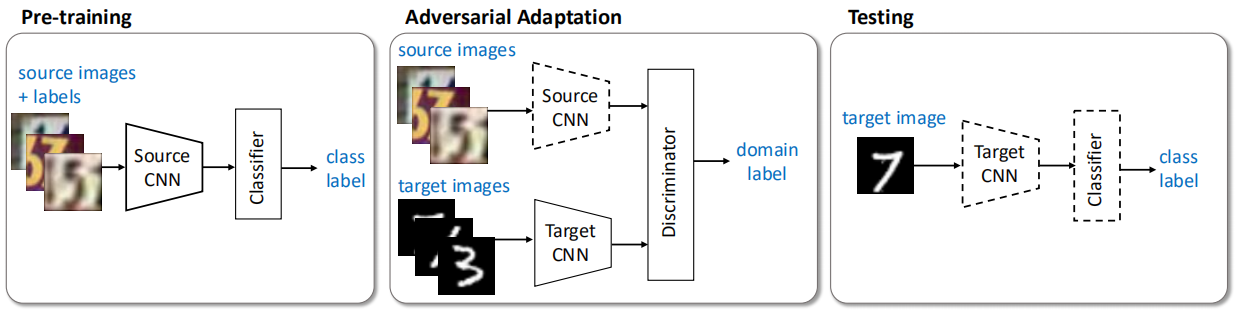
\includegraphics[width=.75\textwidth]{LADDA_theorem1.jpg}
  \caption{ADDA Overview: An overview of standard ADDA architecture. Dashed lines indicate fixed network parameters in the indicated stage.}
  \label{ADDA_overview}
\end{figure*}
The general ADDA approach is presented in figure \ref{ADDA_overview}. There are overall four relatively separated subnetworks within the ADDA model:
\begin{enumerate}
  \item Source encoder network, $M_s$. Source encoder take source data set as input and output the encoded source features.
  \item Target encoder network, $M_t$. Target encoder take source data set as input and output the encoded target features.
  \item Discriminator network, $D$. Discriminator take encoded source features and encoded target features and tries to identify which come from source dataset and target dataset.
  \item Classifier network, $C$. Classifier network take encoded features, from either source or target domain, as input and output the class prediction.
\end{enumerate}

According to work of Eric Tzeng, et al., we can divide the way the model runs into three stages:
\begin{enumerate}
  \item Pre-training. In this stage, we feed source training data, $X_{s}$ for source encoder network and use the output features, $M_s(X_{s})$, to feed classifier network and use cross entropy as classification loss , $L_{c}$:
      \begin{equation}\label{cls_loss}
      \begin{aligned}
        L_{c} & (X_{s}, Y_{s}) =  \\
        &-\mathbb{E}_{(x_s,y_s) \sim (X_s,Y_s)}
        \sum\limits_{k=1}^{K} \mathbb{I}_{[k=y_s]} \log C(M_s(X_{s}))
        \end{aligned}
      \end{equation}
       to train the source network and classifier network. After that, both source network and classifier network are fixed. $K$ is the total number of classes.
  \item Adversarial adaptation. In this stage, we use the idea of GAN to train $M_t$ to generate features, $M_t(X_{t})$, to be similarly distributed as $M_s(X_{s})$. We feed $X_s$ and $X_t$ for $M_s$ and $M_t$ respectively and combination of $M_s(X_{s})$ and $M_t(X_{t})$ for $D$. We in turn optimize $D$ to minimize $L_{D}$:
      \begin{equation}\label{LD}
        \begin{aligned}
        L_{D} & (X_{s}, X_{t}, M_s, M_t) =  \\
                                        &-\mathbb{E}_{(x_s) \sim (X_s)} \log D(M_s(X_{s})) \\
                                        &-\mathbb{E}_{(x_t) \sim (X_t)} \log (1 - D(M_t(X_{t}))
            \end{aligned}
      \end{equation}
      and optimize $M_t$ to minimize
      $L_{t}$:
      \begin{equation}\label{LD}
        L_{t}(X_{s}, X_{t}, D) =
            -\mathbb{E}_{(x_t) \sim (X_t)} \log D(M_t(X_{t}))
      \end{equation}
      $D$ tries to distinguish $M_s(X_{s})$ and $M_t(X_{t})$ while $M_t$ want to deceive $D$. \\
      Our approach is not always quite standard as Eric Tzeng's work. Except that we use fully connected layers instead of CNN for our $X_s$ and $X_t$, we also initialized parameters of $M_t$ using pre-trained $M_s$'s. This is not mentioned in the paper and it is not likely to be feasible in most cases. We can do so because our structure of $M_s$ is designed to be the same as $M_t$. And the measure really help a lot.
  \item Testing. In this stage, we feed $M_t(X_t)$ for $C$ and evaluate the classification accuracy.
\end{enumerate}
    During our practice, we combined the last two stage into one.




\subsection{DANN}
Yaroslav Ganin, et al. proposed a representation learning approach for domain adaptation in their work \cite{DANN1}. DANN can also be viewed as an instance of Eric Tzeng, et al.'s summarization of domain adaptation method. Compared with ADDA, in general, the only difference of DANN is that DANN is an architecture of tied weight sharing.
\begin{figure*}
  \centering
  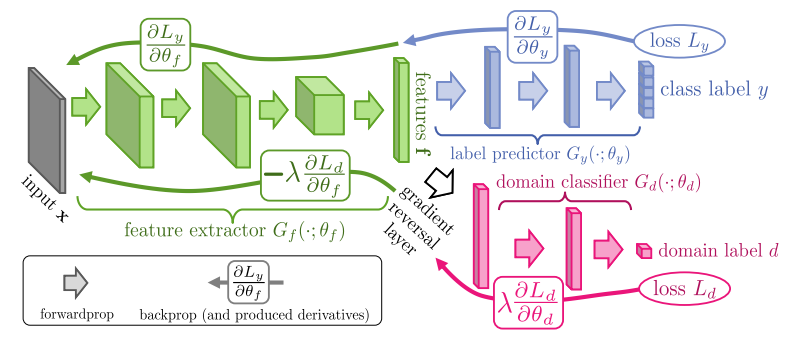
\includegraphics[width=.8\textwidth]{LDANN_theorem1.jpg}
  \caption{DANN Overview: An overview of standard DANN architecture.}
  \label{DANN_overview}
\end{figure*}
The general architecture is presented in figure \ref{DANN_overview}. Domain classifier $G$ of DANN performs similar function as discriminator $D$ of ADDA does. DANN is similar to ADDA but target encoder and source encoder share the same weight weights. In other words, only one feature encoder, $M$, is used within DANN. Thus, we do not go to details of components of DANN and just simply present the way the DANN model work. We will use similar representations as ADDA to make things easy to understand (although they may not be Yaroslav Ganin et al.'s symbols).
\begin{enumerate}
  \item Pre-training. In this stage, we optimize $M$ and $C$ to minimize $L_{C}$.
  \item Adversarial adaptation. In this stage, we feed both $X_s$ and $X_t$ for $M$. By fixing $C$, we optimize $M$ and $G$ to minimize $L_{da}$:
      \begin{equation}\label{dann_da}
        \begin{aligned}
        L_{da} & (X_{s}, X_{t}, M) =  \\
                            &-(\mathbb{E}_{(x_s) \sim (X_s)} \log D(M(X_{s})) \\
                            &+\mathbb{E}_{(x_t) \sim (X_t)} \log (1 - D(M(X_{t}))) \times c_{da} \\
                            &-\mathbb{E}_{(x_s,y_s) \sim (X_s,Y_s)}
                            \sum\limits_{k=1}^{K} \mathbb{I}_{[k=y_s]} \log C(M(X_{s}))
        \end{aligned}
      \end{equation}
      Unlike ADDA, parameters of $M$ and $G$ are updated at the same time. And the loss, $L_{da}$ of DANN is combination of both $L_C$ and $L_D$ of ADDA. There is subtle difference between ADDA and DANN in this stage. $C_{da}$ is a balance factor for classification loss and discriminator loss. $c_{da}$ is not mentioned in the paper, but we use it and find it helps improve our model.
  \item Testing. In this stage, we feed $M(X_t)$ for $C$ and evaluate the classification accuracy.
\end{enumerate}
Also, we combined stage of adversarial adaptation and testing together.

\section{Experiments And Results}
Experiments.

\section{Discussions}
Discussions.

\section{Conclusion}
Conclusions.


\section*{References}

Please number citations consecutively within brackets \cite{b1}. The
sentence punctuation follows the bracket \cite{b2}.

\begin{thebibliography}{00}
\bibitem{ADDA1} Eric Tzeng, Judy Hoffman, Kate Saenko and Trevor Darrel, ``Adversarial Discriminative Domain Adaptation''.
\bibitem{DANN1} Yaroslav Ganin, Evgeniya Ustinova, Hana Ajakan, Pascal Germain, Hugo Larochelle, Francois Laviolette, 
    Mario Marchand, Victor Lempitsky, ``Domain-Adversarial Training of Neural Networks''.
\end{thebibliography}
\vspace{12pt}
\color{red}
IEEE conference templates contain guidance text for composing and formatting

\end{document}
